% Contributions are much appreciated, in order to contribute to this project, head over to this repository:
% https://github.com/bshramin/uofa-eng-assignment

\documentclass[11pt,letterpaper]{article}
\textwidth 6.5in
\textheight 9.in
\oddsidemargin 0in
\headheight 0in
\usepackage{graphicx}
\usepackage{fancybox}
\usepackage[utf8]{inputenc}
\usepackage{epsfig,graphicx}
\usepackage{multicol,pst-plot}
\usepackage{pstricks}
\usepackage{amsmath}
\usepackage{amsfonts}
\usepackage{amssymb}
\usepackage{eucal}
\usepackage[left=2cm,right=2cm,top=2cm,bottom=2cm]{geometry}
\pagestyle{empty}
\DeclareMathOperator{\tr}{Tr}
\newcommand*{\op}[1]{\check{\mathbf#1}}
\newcommand{\bra}[1]{\langle #1 |}
\newcommand{\ket}[1]{| #1 \rangle}
\newcommand{\braket}[2]{\langle #1 | #2 \rangle}
\newcommand{\mean}[1]{\langle #1 \rangle}
\newcommand{\opvec}[1]{\check{\vec #1}}
\renewcommand{\sp}[1]{$${\begin{split}#1\end{split}}$$}

\usepackage{lipsum}

\usepackage{listings}
\usepackage{color}

\definecolor{codegreen}{rgb}{0,0.6,0}
\definecolor{codegray}{rgb}{0.5,0.5,0.5}
\definecolor{codepurple}{rgb}{0.58,0,0.82}
\definecolor{backcolour}{rgb}{0.95,0.95,0.92}

\lstdefinestyle{mystyle}{
	backgroundcolor=\color{backcolour},   
	commentstyle=\color{codegreen},
	keywordstyle=\color{magenta},
	numberstyle=\tiny\color{codegray},
	stringstyle=\color{codepurple},
	basicstyle=\footnotesize,
	breakatwhitespace=false,         
	breaklines=true,                 
	captionpos=b,                    
	keepspaces=true,                 
	numbers=left,                    
	numbersep=5pt,                  
	showspaces=false,                
	showstringspaces=false,
	showtabs=false,                  
	tabsize=2
}

\lstset{style=mystyle}

\begin{document}
\pagestyle{plain}

\begin{flushleft}
Estudiante: Fabio Quimbay\\
Email: fabio.quimbay883@comunidadunir.net\\
Profesor: Miguel Ángel Cabeza\\
\end{flushleft}

\begin{flushright}\vspace{-20mm}

\includegraphics[height=2cm]{logo.png}
\end{flushright}
 
\begin{center}\vspace{0cm}
\textbf{\large PER5786 2022-2023  Física 1 (GFI) - PER5786 2022-2023}\\
 Tema 1 - Magnitudes y unidades físicas
\end{center}

 
\rule{\linewidth}{0.1mm}
%%%%%%%%%%%%%%%%%%%%%%%%%%%%%%%%%%%%%%%%%%%%%%%%%%%%%%%%%%%%%%%%%%%%%%%%

\bigskip
\bigskip

%%%%%%%%%%%%%%%%%%%%
\textbf{Ejercicio 1 propuesto}\\

Sabemos que en un círculo la medida de un ángulo en radianes es igual a la longitud del arco que intercepta (subtiende) dividida por la longitud del radio. Demuestra que el radián es una unidad adimensional.\\

\textbf{Solución:}\\

Un radián es una unidad de medida para los ángulos, definido por el cociente de la longitud del arco de un círculo entre el radio del círculo. Un radián es el ángulo para el cual ese cociente es igual a uno \cite{KA}.

\begin{center}
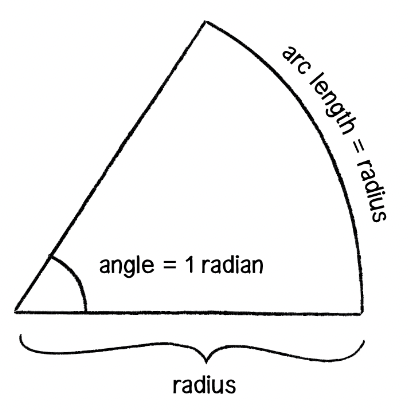
\includegraphics[height=4cm]{radian.png}
\end{center}

La medida $\alpha$ de un ángulo plano es el cociente entre la longitud de cualquier arco s limitado por los lados del ángulo, de centro el vértice del ángulo, y el radio r con que ese arco ha sido trazado: $\alpha$=s/r. Ese cociente es adimensional, por lo que la medida de un ángulo plano es un número real sin unidades. \cite{RM}

%%%%%%%%%%%%%%%%%%%%

\begin{thebibliography}{10}
 \bibitem[Khan]{KA} SHIFFMAN, Daniel., Ángulos y unidades., https://es.khanacademy.org/computing/computer-programming/programming-natural-simulations/programming-angular-movement/a/angles-and-units
 \bibitem[Redondo]{RM} F. R. Quintela y R. C. Redondo Melchor. Diccionario de Ingeniería Eléctrica. Universidad de Salamanca.
https://electricidad.usal.es/Diccionario
\end{thebibliography}

\end{document}

